\section{Appendix}
%% Figs
\renewcommand{\thefigure}{S\arabic{figure}} % Changes the figure numbering to S1, S2, etc.
\setcounter{figure}{0} % Resets the figure counter
\begin{figure}[h!]
    \centering
    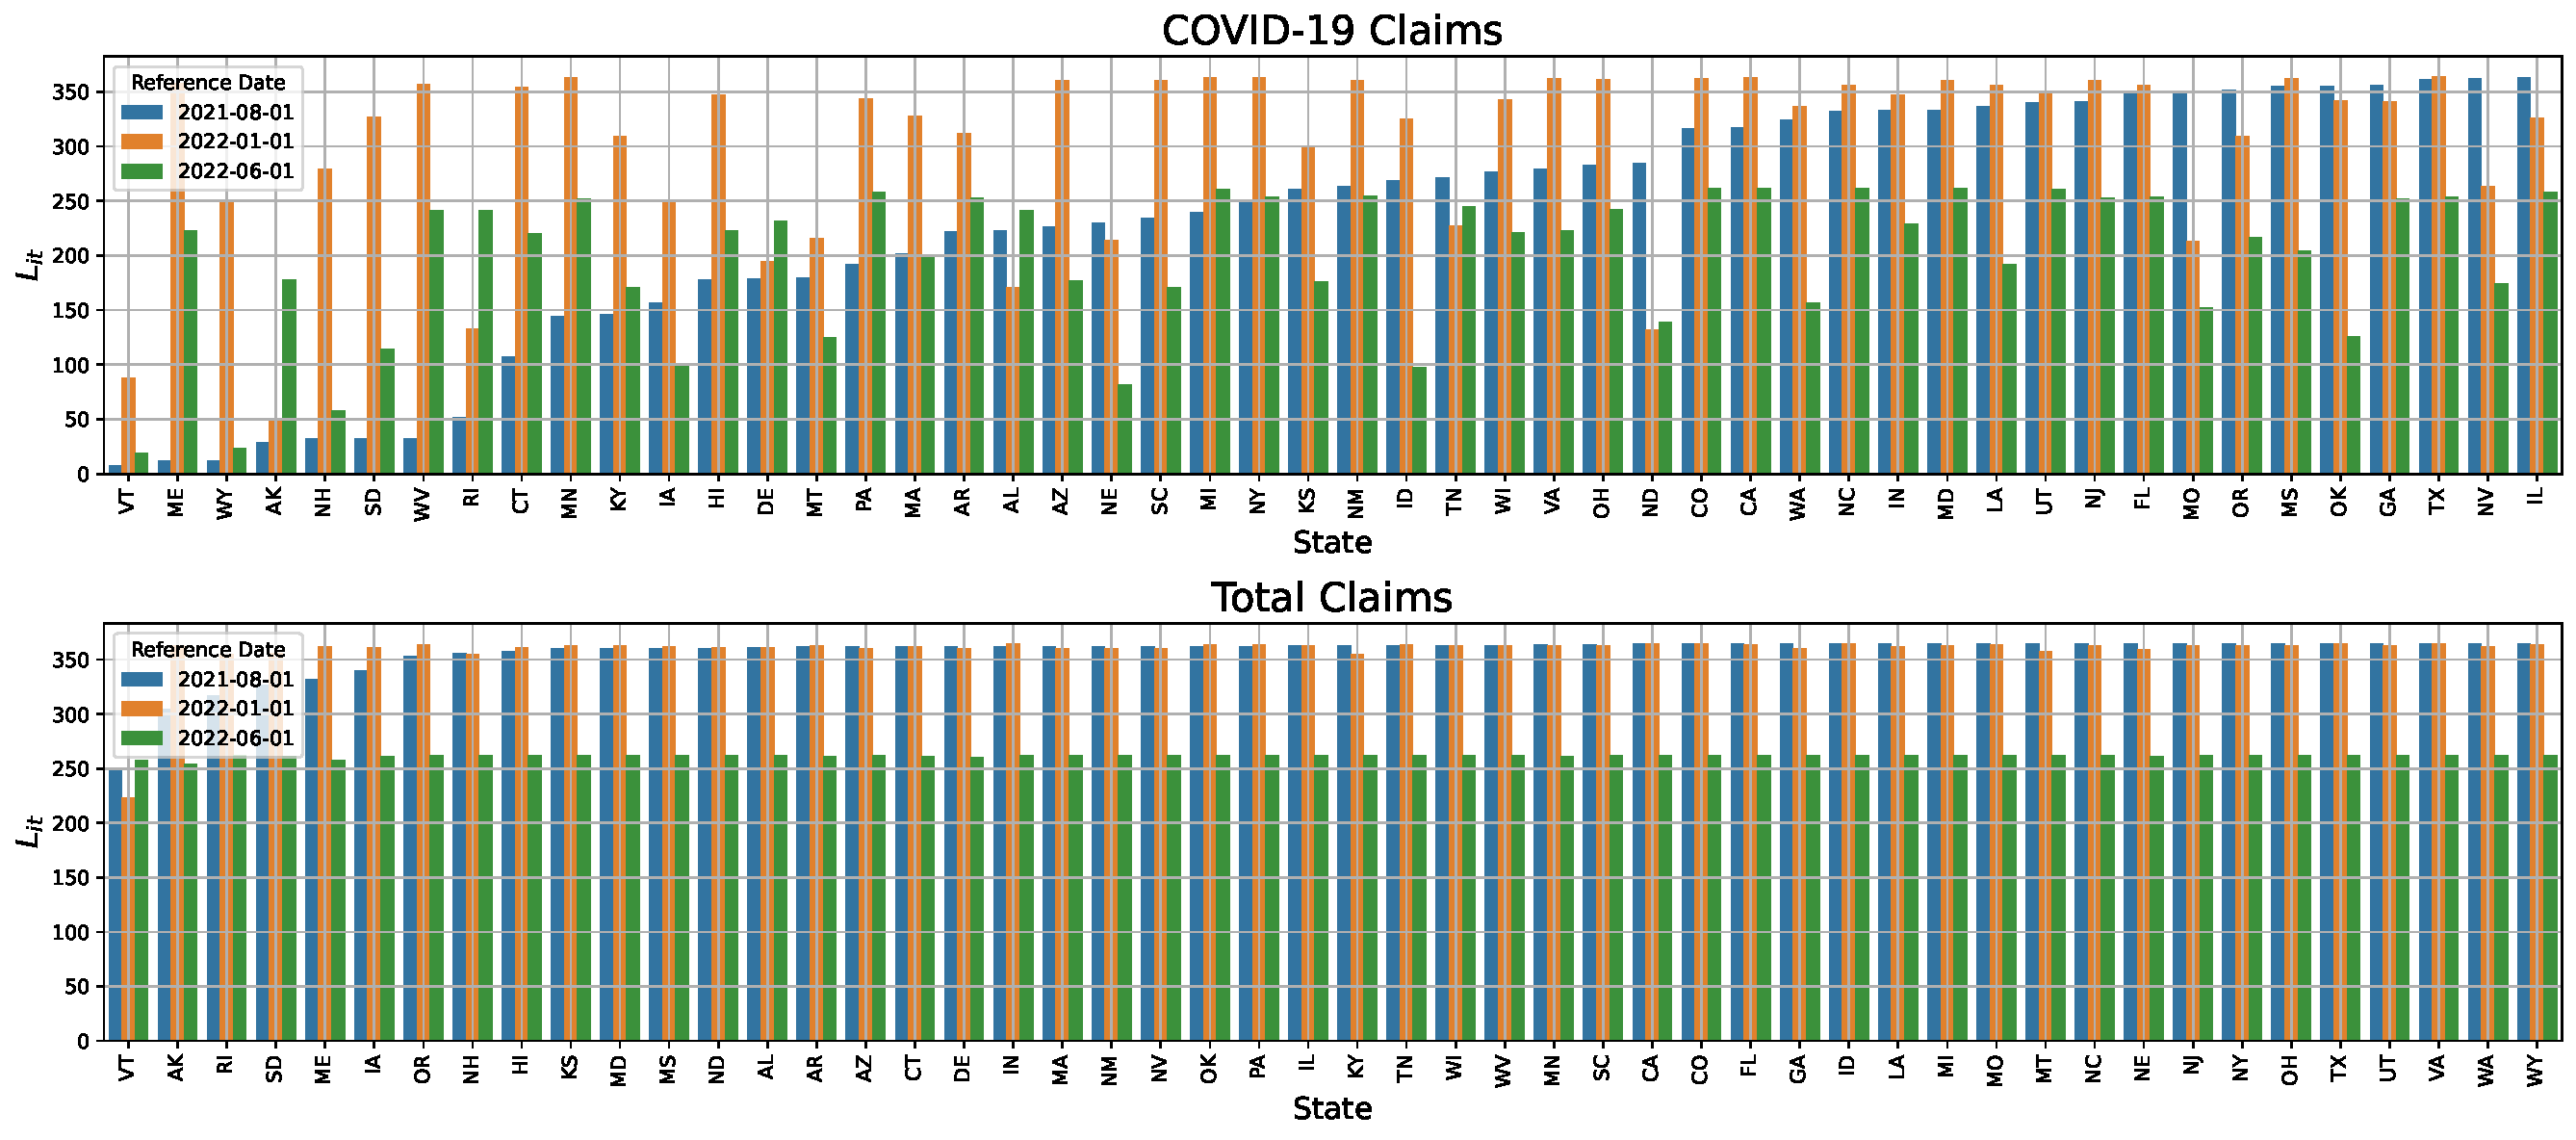
\includegraphics[width=\textwidth]{figs/Lit_examples.pdf}
    \caption{\emph{Top: comparison of the smallest lags required for convergence across states, displayed for samples of different reference dates, based on CHNG outpatient COVID-19 insurance claims. Bottom: as in the figure on the top, but based on CHNG outpatient total insurance claims.}}
\end{figure}


$L_{it}$ is not uniformly random, the distribution of \%reported indicates that substantial effective revisions are typically made within the first two months. As a result, we step back and introduce a target lag $L$ and using $Y_{itL}$ as the projection target. For any location $i$ and reference date $t$, we assume that $$\mathbf{E}[\frac{| Y_{it} - Y_{itL}|}{Y_{it}}] \leq \epsilon $$ The larger the target lag $L$ is, the smaller $\epsilon$ can be. In essence, the selection of the target lag $L$ involves a trade-off between timeliness and accuracy. Out of practical considerations and understanding of CHNG outpatient data, we set $L=60$ henceforth in our real-time data revision correction experiments.
\clearpage
